\documentclass[paper=a4,draft=false]{scrartcl}
\usepackage[english]{babel}

\usepackage{apacite}
\usepackage{endnotes}
\usepackage{url}
\usepackage{fixltx2e}
\usepackage{appendix}
\usepackage{booktabs}
\usepackage{caption}
\captionsetup[subfigure]{labelformat=empty}
\usepackage{subfig}
\usepackage[utf8]{inputenc}
\usepackage{fullpage}

% Set vertical line spacing
\usepackage{setspace}
\setstretch{1.5}

\usepackage{amsmath}
\usepackage{amssymb}
\usepackage{color}
%\usepackage{latexsym}
% Surround parts of graphics with box
\usepackage{boxedminipage}
% Package for including code in the document
\usepackage{listings}

% If you want to generate a toc for each chapter (use with book)
\usepackage{minitoc}

% This is now the recommended way for checking for PDFLaTeX:
\usepackage{ifpdf}
\newcommand{\note}[1]{{\textbf{Note:} \color{blue} #1}}
%\newif\ifpdf
%\ifx\pdfoutput\undefined
%\pdffalse % we are not running PDFLaTeX
%\else
%\pdfoutpu68=1 % we are running PDFLaTeX
%\pdftrue
%\fi

\ifpdf
\usepackage[pdftex]{graphicx}
\else
\usepackage{graphicx}
\fi

% declare non-metalanguage data
\newcommand{\lingform}[1]{\emph{#1}}
\newcommand{\term}[1]{{\bf #1}}
\newcommand{\scare}[1]{``#1''}
\newcommand{\meta}[1]{\textsc{#1}}
\newcommand{\code}[1]{{\tt #1}}

\title{Graphical representation of document similarity using named entity recognition and lexical similarity}
\author{Todd Shore, Carsten Ehrler, Michal Richter and Yevgeni Berzak}
\date{\today}

\begin{document}

\ifpdf
\DeclareGraphicsExtensions{.pdf, .jpg, .tif}
\else
\DeclareGraphicsExtensions{.eps, .jpg}
\fi

\maketitle
\tableofcontents

\begin{abstract}
\end{abstract}

\section{Introduction}\label{sec:introduction}
\subsection{General Description}
\label{sec:general_description}
The availability of historical documents in digital form has been constantly increasing in recent years. 
Digitalization of sources is extremely valuable for historians, as it contributes to preservation, facilitates 
accessibility and enables exploiting computational methods for the benefit of historical research. Despite the growth 
of digitalized historical data, available collections are rarely accompanied by tools which significantly facilitate the 
work of historians. If available at all,  interfaces typically include a simple keyword search, providing the user a list 
of documents that match his query. 

Though such tools can indeed spare valuable time dedicated to manual work, 
they are far from exploiting the full power and flexibility that state of the art technology has to offer. 
Moreover, provided systems are usually generic, and rarely address the specific needs of researchers in the historical domain. 
This situation calls for development and adaptation of NLP techniques for historical data, as well as for creation of user interfaces 
that would enable historians to use this technology effectively for their needs. 

This project addresses both aspects the current shortage. We take up the algorithmic challenge by applying and tailoring NLP tools 
that extract information relevant for historians and link between historical documents according to similarity with regard to this information.
The need for intuitive user interfaces is addressed by providing an interactive graphical tool that enables historians without 
computational background to use relevant NLP techniques and present their outcome. This twofold approach aims at improving the chances of 
historians working with sources to find information that is relevant for their research goals.

The core idea of our approach is to extract historically relevant information, such as persons, locations and organizations mentioned in each document,
and then use this information to determine similarity between documents. Similarity according to historically relevant information
can then be interpreted in terms of links between documents and be represented graphically for various uses.

We introduce an interactive graphical system for powerful search and navigation through a collection of historical documents. 
We exemplify our approach on the \citeA{CastroDB} (CSDB), a collection of
speeches and other documents by Fidel Castro. Our system includes keyword and metadata search with automatic query 
expansion for named entities. 
Retrieved documents are presented in a table as well as in an interactive graph, in which nodes represent 
documents and edges represent links between documents. Documents are linked according to the amount of NEs each has in common, by the degree of lexical
similarity, or by both measures. This representation is designed to support the identification of groups of documents which revolve around similar topics as well as the exploration of more specific relations between any subset of presented documents. The system also enables the user to receive a local perspective on a 
specific document and present its most strongly connected neighbors, thus serving also as a recommendation tool. 

Underlying the system are various computational methods and tools for text processing, 
information storage and retrieval, named entity recognition (NER), co-reference resolution (CRR), 
data visualization and others. In the following section, we provide an overview of the specific processing subtasks involved and the functionalities of the system.

\subsection{Subtasks}
\label{sec:subtasks}
\subsubsection{Preprocessing Steps}

Several processing tasks were performed in the course of implementation of the project. Following is an overview of the steps involved. An in-depth description of each step is provided in section \ref{sec:main_part}.

\begin{description}
\item[Reading Data] All documents from the CSDB were retrieved. Meta-data provided for each document was extracted from its header.
\item[Storing Data] Documents were stored in a MySQL database, and a data model was created in order to allow efficient retrieval of documents by metadata.
\item[NER] A NE recognizer was used to identify \meta{Persons}, \meta{Locations} and \meta{Organizations} in each document.
\item[Document Indexing] Documents were indexed in four different manners in order to support document retrieval and serve as input for similarity calculations--- Three indexes were based on the three types of identified NEs, while the fourth indexing method was based on global vocabulary. Terms were weighted according to both TF and TF/IDF measures.
\item[Co-reference Resolution] In order to avoid treating linguistic form variations as different entities, we implemented an approximation of a CRR system, focusing on aliasing (the identification of linguistic-form variations).
First, similarity matrices between all NEs of the same type in the database were calculated using a $p$-spectrum string kernel.
Afterwards, the similarity matrices were multiplied by the documents matrix. As a result, each document representation was boosted by all form 
variations of the NEs that it contains.
\item[Calculation of Document Similarity] Document similarity matrices were created according to two different similarity measures. 
Similarity was computed separately according to NEs and lexical overlap. 
A link can be established between a pair of documents if their similarity passes a certain threshold. 
The strength of the link is determined by the strength of the similarity.
\end{description}

These processing steps created the infrastructure for a graphical user interface that provides several
functionalities described in the following section.

\subsubsection{Functionalities of the Application}
\begin{description}
\item[Document Retrieval Engine] Using the data model and precomputed indexes, an engine for document retrieval was implemented. 
The engine allows querying the database with keywords. The engine also allows filtering and querying according to specifications on metadata, e.g.\ a period of time, type of document and others. 
\item[Graphical Representation of Documents] Documents retrieved from the database are presented as nodes of a graph. The size of the node corresponds to its relevance for the query, its shape to the type of the document. We retrieve the similarity measure for each pair of documents, and link them with an edge if the similarity crosses a adjustable threshold. The thickness of edges reflects the strength of the similarity between two documents.
\item[Functionalities for Exploration of the Collection] We provide an interactive environment that enables the user to navigate through the documents in an effective way. Among the implemented features are viewing the list of NEs of a particular document; viewing common NEs for several documents; presenting the content of a document with the NEs marked; marking the most similar documents to a specific document; isolating the neighbors of a document up to a specified depth; and manipulating edges representation for thresholds, absolute/relative similarity and options for $k$-Means or Chinese Whisper clustering of the documents.
\end{description}

A detailed description of each functionality is provided in section \ref{sec:gui}. In the following, we present the interest of our application for historical research. 

\subsection{Motivation: Working with Collections of Historical Documents}
\label{sec:motivation}
One of the major tasks of historians consists of working with sources that often come in the form of historical documents. 
Such documents have numerous usages in the various branches of historical research. Some of these are related the quest of revealing 
general trends and patterns about a historic period or personality, while others focus on finding specific details and pieces of historical 
information. Historical documents serve both for the formulation of historical hypotheses and for their validation and rejection efforts. 

While the amount of written accounts about ancient history is well-known and relatively limited, researchers of modern times often have to 
face an abundance of historical written materials. Dealing with large collections of documents introduces additional challenges for historians. 
In particular, the focus is often shifted to the identification and retrieval of documents that might be relevant for the interests of 
historians. Furthermore, identifying trends as well as implicit and explicit links between documents becomes an extremely difficult task to 
perform manually.

Our system is designed to support the work of the historian with electronic sources in several ways, specifically with large collections of documents such as the CSDB. Following are some of aspects of our system that are likely to be appealing for historians.

We focus on automatic markup of NEs. In particular, we identify \meta{Persons}, \meta{Organizations} and \meta{Locations}. All three bear potential 
interest for historians, both in terms of discovering of new entities and identification of known entities. 

Retrieval of documents that contain known NEs or general keywords is done automatically. Documents containing form variations of 
the entities appearing in the query can also be retrieved, enabling historians to receive documents that might be relevant for their interests 
but do not appear in their query.

Our retrieval mechanism and graphical interface incorporates metadata, if such is provided with the documents in the collection. 
Using metadata extends the flexibility of the search and allows a more informative graphical presentation of query results.

We present links between retrieved documents based on the overlap of NEs in each document as well as general lexical overlap. These links can be valuable in many scenarios. 
For instance, if the historian is interested in a specific document, he or she can easily identify which other documents contain similar named 
entities or similar vocabulary. This feature not only helps with the discovery of explicit information about NEs in the 
collection, but can also provide useful generalizations with regard to documents that potentially deal with similar, sometimes implicit 
topics to those of the document of interest.   

Providing a graphical representation of the query results also supports the historian in inferring global statements about the collection or 
one of its subsets. In particular, one can identify groups of highly interconnected documents. Identified dense regions are likely to reflect 
different kinds of topics and might be correlated to various parameters, such as time and location. Absence of links and identification of 
``stand-alone'' documents can also be highly informative, as they can indicate unique content. 

Our system aims to be both intuitive and simple while allowing considerable amount of flexibility. It enables users to adjust many of the 
parameters such that they would best suit their needs. A historian who has an intuition that any sort of links between the documents might 
be relevant for him, may adjust the similarity threshold for presenting edges to be very low and display even relatively-weak links between documents. On the other hand, if only tight connections 
are desired, the threshold can be raised, revealing only relatively-stronger links. Other operations on the graph such as switching from NE to lexical similarity, adjusting 
thickness of edges to reflect different degree of similarity, setting links according to TF/IDF measures and others have explicit textual 
interpretation and the potential to help to the user achieve his goals. 

Finally, our system is designed to make retrieval and navigation through the collection easy and enjoyable. We provide text viewing 
possibilities, and graph manipulation operations such that the user would be able to explore the collection effectively and with minimal effort.

\subsection {Background and Previous Work}
\label{sec:nlp_background}

Our work lies within the areas of NLP, IR and Knowledge Domain Visualization.
It involves several well-known NLP and information retrieval (IR) tasks as well as topics from information visualization and user interfaces. 
We tackle these tasks with a combination of off-the-shelf tools, implementing and adapting established models, and by introducing new methods 
that suit our purposes. In the rest of this section, we provide a general overview of the different tasks and frameworks involved in our 
project, review relevant previous research and relate it to our implementation. 

An important NLP task we face is NER. This task refers to the identification and classification of rigid designators, 
typically proper names \cite{NEsurvey2009}. Three well-studied types of NEs are \meta{Persons}, \meta{Organizations} and \meta{Locations}. 
As mentioned previously, all three are important for the historical domain. While early studies in NER focused on designing 
hand-crafted rules, recent studies and state-of-the-art tools apply statistical and machine learning techniques. For such tools, 
good feature selection has proven to be crucial, and often more important that the model itself.  
To recognize NEs in our collection we apply the Stanford Named Entity Recognizer (SNER) \cite{sner}. It is based on Conditional Random Fields (CRF), 
uses a wide range of features and is available with pre-trained models.  For a detailed description see section \ref{sec:stanford_named_entity_recognizer}.

Another branch of NLP research relevant for our work is CRR, involving the task of determining which phrases refer to the same extra-linguistic entities in a text or a collection of texts.
Following the relative success of the algorithm and features proposed in \cite {soon2001coreference}, machine learning 
with an emphasis on feature engineering has been the predominant approach for this task. CRR is widely 
recognized as an extremely complex problem and existing tools such as BART \cite{bart} achieve only moderate accuracy (an F-score of roughly 65\%). Due to the limitations of existing technology and the nature of our task we restrict ourselves to multi-document aliasing, namely recognizing variations in the form of the same entity in a collection of documents. Our approach is based on string similarity, 
which we approximate using a p-spectrum string kernel \cite{kernels2004}. We describe our co-reference approach in section \ref{sec:aliasing}.

Our implementation of the document retrieval modules and linkage of documents according to similarity relies heavily on standard techniques 
and measures used in IR, and specifically on the vector space model \cite{ir2008}. We adopt and adapt techniques for 
document indexing \cite{indexing1999}, vector space term weighting \cite{jones2004}, \cite{salton1971}, query extension and determining query-document and 
inter-document similarity. 

From a wider perspective, the project can be located within the field of Domain Knowledge Visualization. This field revolves around visualization
techniques of domain structures, in particular for scientific domains. Its notable applications are mapping structures of domains and supporting
IR and information classification.
The general process flow of visualizing domain knowledge as described in
\cite{visualizing2003} is the following: 
\begin{enumerate}
\item Data extraction 
\item Definition of unit of analysis 
\item Selection of measures 
\item Calculation of similarity between units 
\item Ordination or assignment of coordinates to units 
\item Use of resulting visualization for analysis and interpretation.
\end{enumerate}
Our workflow conforms exactly to these categories. We use NEs and general vocabulary as extracted data, documents as units of analysis, measure and calculate similarity with Manhattan and cosine distances, order documents according to these measures, and finally visualize the results as a graph.
From this perspective, the NLP module is a sub-component which falls within the data extraction step. Extracting NEs is of critical importance
here, as this type of information is extremely relevant for historical documents in contrast to in some other domains.  

More specifically, our model can be regarded as a special case of a pathfinder network \cite{schvaneveldt1990pathfinder}.
Modeled as a pathfinder networks a collections of documents may be represented as a graphs representing the relative proximities of each objects to each other. 
Objects are represented as nodes and proximities between objects are represented as links between nodes, where only the strongest links according to a adjustable proximity threshold are taken into consideration. Proximity can have several interpretations, one of them being similarity.
Degrees of similarity between two objects are typically modeled in the length their links. The more similar two objects are, the shorter their link.
In our implementation, however, degree of similarity is divided into three categories and reflected by the thickness of each line.


\section{Main Part}\label{sec:main_part}
\note{Detailed description of the subtasks that your system performs: 
how does it tackle these subtasks? 
why did you choose this approach? 
did you encounter specific problems that you had to solve? 
how did you solve them?}

<<<<<<< HEAD
\subsection{Data}
\label{sec:data}

\subsubsection{Description of the Castro Archive}
\label{sec:description_of_the_castro_archive}
\note{technical details on the database, statistics, typical structure of a document}

\subsubsection{Reading and Storing the Data}
\label{sec:reading_and_storing_the_data}
\note{reading the data, creating MySQL database, creating data model}

At a first step we used a \texttt{shell}\footnote{http://tiswww.case.edu/php/chet/bash/bashtop.html}
script and \texttt{wget}\footnote{http://www.gnu.org/software/wget/} to download the complete castro
speech database. The actual speech data consists of a set of static webpages sorted by year into
folders. In a second processing step we parsed these html-files and extracted the actual content of
each file and its meta-information into textual format. To this end, several \texttt{shell} and
\texttt{python}\footnote{http://www.python.org/} scripts have been written.

The extracted information serves as the basis for the consecutive analysis and processing steps. In
order to provide structured access to the meta-information we developed a
\texttt{perl}\footnote{http://www.perl.org/} script to convert the meta-information for each
document into an entry in a \texttt{mysql}\footnote{http://www.mysql.de/products/enterprise/}
database. For every document, the database provides the following information
\begin{itemize}
 \item{\textsc{Author:} Name of the author of the document.}
 \item{\textsc{Location:} The place the document orginated.}
 \item{\textsc{Headline:} The headline of the document.}
 \item{\textsc{Date:} The date the document orginated.}
 \item{\textsc{ReportDate:} The date th3e content of the document appeared in written from.}
 \item{\textsc{Type:} There are several different types of documents in the databse. E.g.
 \texttt{SPEECH}, \texttt{INTERVIEW}, \texttt{ARTICLE}, etc.}
 \item{\textsc{Header:} Additional meta-information}
 \item{\textsc{Source:} The source where this document appeared in written form the first time.}
\end{itemize}
In addition to this information, we later enriched the database with the extracted named entities
(see \ref{sec:named_entity_recognition}) for each document. The columns \textsc{Persons},
\textsc{Places}, \textsc{Organizations} have been added and each field contains the bulk information
of the identified named entities as a comma separated list. Although this representation is is not
the most elegant and optimal solution, the derived database provides sufficient performance and
usability for the task at hand.

\subsection{Named Entity Recognition}
\label{sec:named_entity_recognition}
Please recall, that our ultimate goal is to come up with a cross-document recommendation system for
the castro speech database. Therefore, we need an appropriate metric on between document
similarity that serves as a basis for the recommendation software.

Our first idea was to use proper \textit{co-reference resolution}, e.g. provided by
\texttt{BART}\footnote{http://www.bart-coref.org/} software \cite{bart}. In this case, document
similarity is a function of the number of co-references that appear between two docuemnts. However,
in the end we decided to drop this approach because of the overall complexity and the tight time
constraints. In general, between document co-reference resolution far from an easy task. The castro
database though has some nice properties that allow for a more straightforward solution. For this
dataset, the domain is rather limited and the number of distinct topics should be small. Hence, we
came up with the idea to base the similarity measure on smoothed co-occurences of named entities.

The next step in the pre-processing chain is thus the execution of named entity recognition followed
by a smooting of the features in the vector space induced by the named entities using kernel
methods (see \ref{sec:string_kernel}) \cite{string_kernel_coref}.

\subsubsection{The Stanford Named Entity Recognizer}
\label{sec:stanford_named_entity_recognizer}
\note{details on the tool}

\subsubsection{Recognizing Named Entities in the Castro Archive}
\label{sec:recognizing_named_enitiies_in_the_castro_archive}
\note{identifying names, locations and organizations in the Castro documents,
input/output examples, evaluation??}

\subsection{Representing Documents in Vector Space}
\label{sec:representing_documents_in_vector_space}

\subsubsection{Indexing and Term Weighting}
\label{sec:indexing_term_weighting}
\note{description of the 4 different representations, tf/tfidf with motivation and
interpretation for each, examples}

\subsubsection{Aliasing with String Kernels}
\label{sec:aliasing_string_kernel}

\note{motivation, description of the algorithm to create similarity matrixes between NE's,
smoothing document representations with Kernel matrix as aliasing}

\subsection{Information Retrieval}
\label{sec:information_retrieval}

\subsubsection{Keyword Search}
\label{sec:keyword_search}
\note{description of the functionality, use of string kernels for query expansion }

\subsubsection{Metadata Search}
\label{sec:metadata_search}
\note{general description of the functionality}

\subsection{Computing Similarity between Documents}
\label{sec:computing_similarity_between_documents}
\note{calculating similarity matrice.}

\subsection{Graphical Representation}
\label{sec:graphical_representation}
\subsubsection{Computing Graph Layouts}
So far we have described how nodes and edges of the graph are obtained from documents and their
similarity. In order to display the graph, a graph layout (two dimensional representation of the
graph) must be determined. If the vector representation of the document is only two dimensional,
then it is straightforward to obtain the graph layout just by using the features as two dimensional
coordinates. However, the documents in our model are represented by vectors with several thousands
of dimensions. The problem of reducing the dimensionality, is usually not solved by mapping
from high dimensional vector space to the low dimensional vector space but by using algorithms that
solve the problem of graph layouting directly using only the properties of the underlying graph
(nodes and edges together with their weights).

The layouting algorithm that was used in this project belongs to the popular class of force-based
layout algorithms which are based on physical modeling. An Edge is considered a spring and
the nodes are considered to be electrically charged particles (i.e.\ with equal signed charge such
that they repel each other) The optimal length of the springs is set in advance. Springs whose
length is larger or smaller than their optimal length exert a force that acts on the connected
nodes. In each iteration of the layouting algorithm, nodes are moved according to the resultant
force
that acts on them. After some time the position of the nodes becomes (quasi) stationary and the
system get into a local equilibrium state.

The described class of force based layout algorithms subsumes various algorithms with different
properties. However, they all perform variations of force-field energy minimization by iterative
approximation schemes. In this project the very basic algorithm as it is described in the previous
paragraph was used.

\subsubsection{Jung Graph Framework}
For the purpose of graph layouting, graph painting and user-graph interaction, the
\texttt{Jung\footnotemark{http://jung.sourceforge.net/} - java universal network/graph framework}
was used. It provides great flexibility in adjusting the graph appearance. Several so-called
transformers which affect node and edge label appearance can be plugged together to result in the
aesthetically pleasant appearance. \texttt{Jung} also provides predefined classes that allow for
easy interaction with the user. Functionalities for graph translation, zooming, node selection, node
transposition and other features can be achieved with minimal programming effort. One notably
strong point of the library is its template based design with the possibility to include several
plug-in components such as rendering and transformers that affect the resulting appearance of the
graph.

However there are some aspects of the \texttt{Jung} library, that were annoying fro the project.
First, it is difficult to achieve certain low level functionalities, like e.g.\ monitoring the
on-screen position of a fixed point while translation of the graph was performed. Secondly, several
operation are implemented in a circumstantial way. For example, in order to change the color of
one node the whole graph must be redrawn and during this process all active visualization
transformers are applied on each graph object.When we used the default implementation of the
\texttt{Jung} visualization class, the application consumed more then 50\% of the processor time
even though there was no ongoing user interaction or computation task (this depended on the size of
the presented graph --- the statement holds for graph with 25 nodes about 50 edges). By extending
the standard \texttt{Jung VisualizationViewer} class and overriding several functions, the issue of
unnecessary graph redrawing was resolved and accordingly the problem of the low gui performance.

\subsubsection {Querying Functionalities}
\label{sec:querying_functionalities}
The nodes of the graph are generated from the results of a database query supplied by the user, who
can search either by keyword, by NE, or by a combination of both in the same query. Likewise, the
user may select a range of years to search in (e.g.\ retrieve documents occurring between
\code{1970} and \code{1975}), as well as select only certain types of documents to be searched
(e.g.\ retrieve only documents of type \meta{Speech} or \meta{Interview}). The documents most
relevant to the current query are displayed, the number of the documents displayed being specified
by the user (e.g.\ display the \code{25} most relevant documents), and edges connecting each
document are drawn based on the similarity measures relating each document to each other.

\subsubsection {Presenting Results}
\label{sec:presenting_results}
After submitting a query, a table of query results is displayed and a graph corresponding to the
results is drawn, in which the relevance measure of each document to the current query is
represented by the absolute size of the node representing the document in question: The larger the
node, the more relevant it is to the current query. The type of document represented by the node is
represented by its shape, e.g.\ \meta{Speech} $\rightarrow$ star, \meta{Meeting} $\rightarrow$
pentagon. The edges linking the nodes of the graph represent the strength of similarity the of the
two documents represented by the nodes.
	
\subsection{Combining It All: User Interface} 
\label{sec:combining_it_all:_user_interface}
The query functions, graph and display functions are integrated into a single graphical front-end relying primarily on the mouse for user input. The graph representation is dynamic and interactive, able to be navigated through by the user in order to obtain detailed information regarding the document database.

\begin{figure}[ht]
\centering
\caption{GUI}
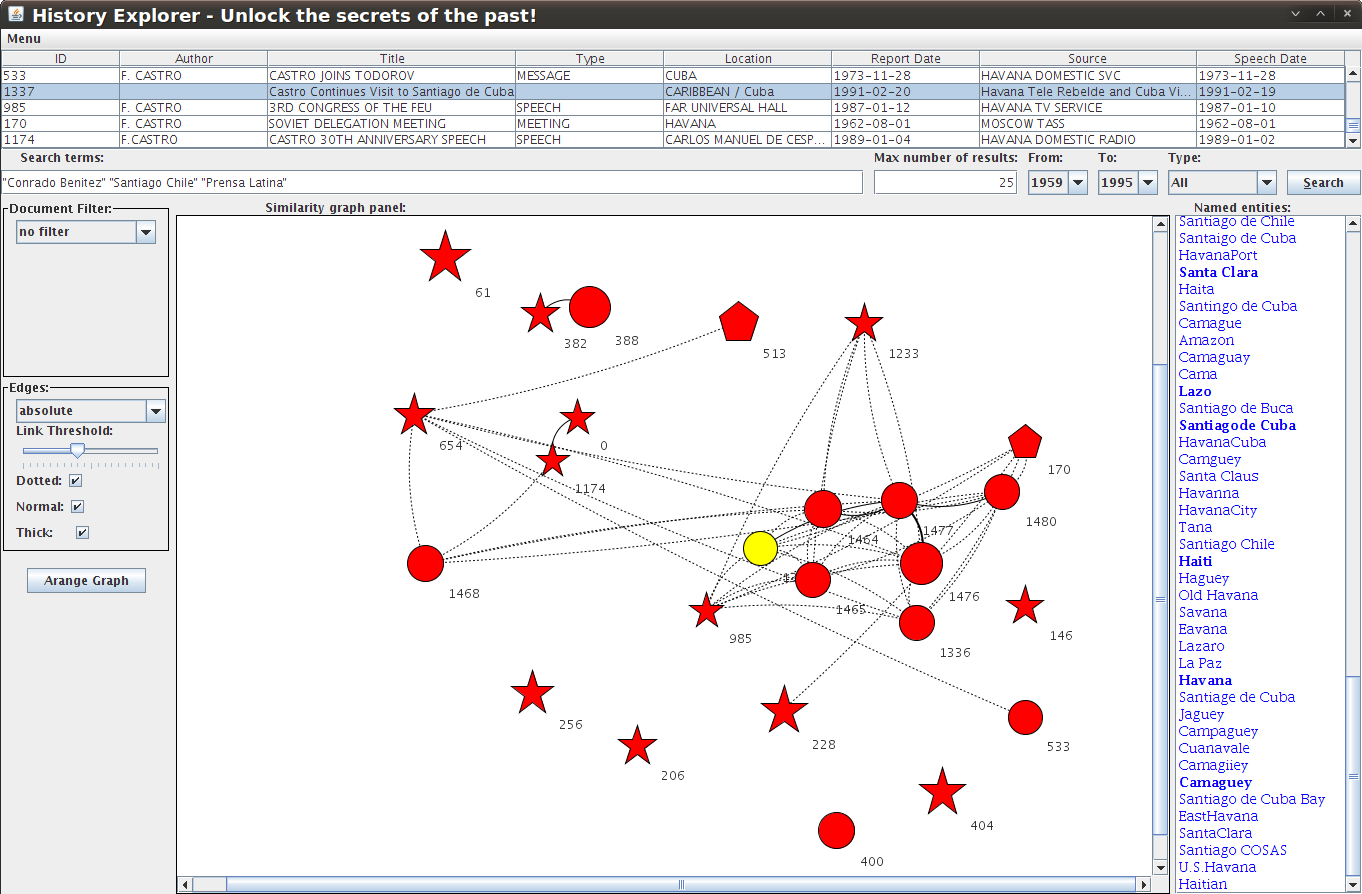
\includegraphics[width=160mm]{gui.png}
\end{figure}

\subsubsection{Search Function}
\begin{figure}[ht]
\centering
\caption{Search query}
\subfloat[][~\hfill{\tiny Version $<$\code{2010-04-02}}]{

\includegraphics[width=160mm]{search.png}
}
\end{figure}

Search terms are entered in the query form (item 1 in the figure above)\footnote{Unless otherwise mentioned, the version depicted is \code{2010-04-02}.}: Entering any term will return both NEs and also keywords sharing the exact form (not case-sensitive)--- For instance, entering \lingform{committee} will both return exact instances of \code{committee} in the document itself, and will return NEs similar to \lingform{committee} based on the string kernel similarity measure, e.g.\ \lingform{Central Committee} and \lingform{Central Committee of the Cuban Communist Party}. Multi-word terms are denoted in double quotes, e.g.\ \code{"Central Committee"}. The maximum amount of query results can be adjusted (item 2): For example, entering a value of \code{10} will return ten documents most relevant to the query. The set of years searched between is also modifiable specified by (item 3), as well as the type(s) of documents searched (e.g.\ \code{Speech}, \code{Interview}) (item 5). Once the criteria are entered, the query is run by selecting item 5.

\paragraph{Presentation}
The results of the current query are displayed both in a table of results and in a graph displayed in the main window.

\subsubsection{Visualization of Results}
\begin{figure}[ht]
\centering
\caption{Query Results Table}
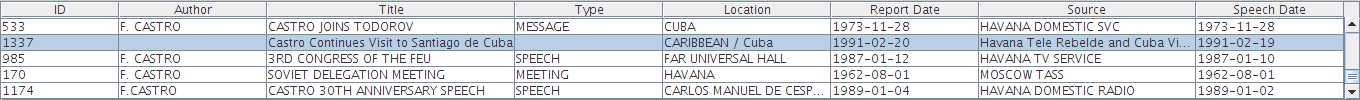
\includegraphics[width=160mm]{table.png}
\end{figure}

In the table, the documents are displayed in rows sorted by their relevance to the query in descending order. The metadata associated with each document is displayed in columns. If there was no metadata retrieved for a document, the entry for the data is empty or \code{NULL}.

\begin{figure}[ht]
\centering
\caption{Document Similarity Graph}
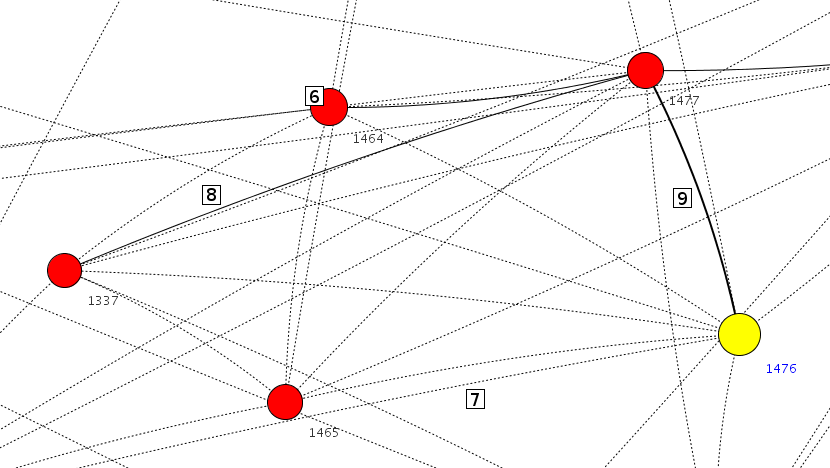
\includegraphics[width=80mm]{nodecloseup.png}
\end{figure}

In the graph, each document is represented by a node (item 6). The relevance of the document to the query is represented by the size of the node: The larger the node, the more relevant the document is to the submitted query. The edges between the nodes represent similarities between the documents based on the similarity of the two documents based on the NEs each contain and their aliases according to the string kernel measure. The stronger the similarity connection, the heavier the line weight of the edge drawn. There are three line weights: ``dotted'' (item 7), ``normal'' (item 8) and ``heavy'' (item 9), in ascending order of the level of similarity they represent. The graph can be scaled in real-time by zooming in and out with the scroll wheel. Furthermore, it is able to re-arrange the position of each node in the graph by clicking and dragging them in order to optimize the view of the graph manually. The graph can also be set to re-arrange the nodes automatically by clicking ``Arrange Graph''. By pressing CTRL and clicking on a node, the view will be centered on the said node automatically.

\paragraph{Navigation}
Selecting a document either through its corresponding entry in the table or node in the graph with the mouse or keyboard highlights it and displays the NEs in the document in a sidebar. The NEs in a particular document and their string kernel-based aliases are displayed in the sidebar: Boldface entries represent NEs in the given document, while the non-boldface entries represent NEs similar to the boldface NEs in the document according to the string kernel similarity measure. For example, the NE \textbf{\lingform{Castro}} may also return the similar NEs \lingform{Fidel}, \lingform{Fidel Castro} and \lingform{Dr.\ Fidel}. The type of the NE (e.g.\ \meta{person} or \meta{organization}) is represented by the color of the text, e.g.\ red for \meta{Persons}, green for \meta{Organizations} and blue for \meta{Locations}. It also is possible to select multiple documents, e.g.\ by holding SHIFT and clicking on multiple nodes/table entries, or by clicking and dragging the mouse to create a selection box encompassing the nodes/table entries to be selected. When multiple documents are selected, the entries displayed in the sidebar are those that are common to all selected documents.

\begin{figure}[ht]
\centering
\caption{Node Context Menu}
\subfloat[][~\hfill{\tiny Version $<$\code{2010-04-02}}]{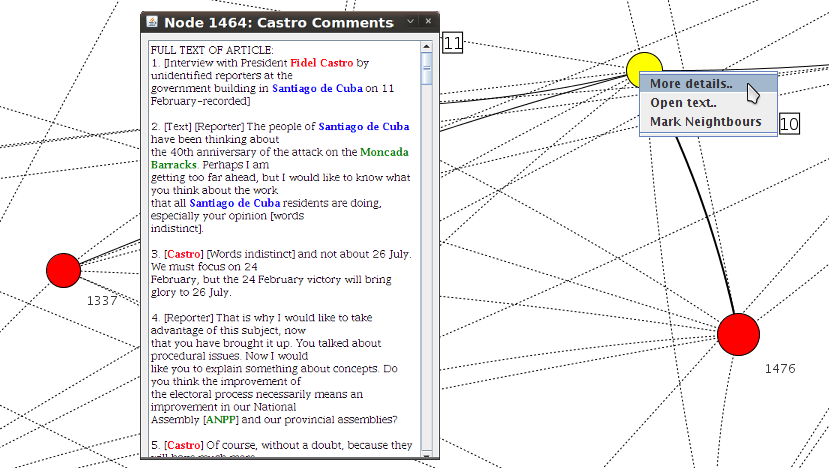
\includegraphics[width=80mm]{nodeclick.png}}
\end{figure}

In addition to viewing document metadata in the query results table, the user may to view the metadata of the document associated with a particular node (e.g.\ document \meta{Type}, \meta{Date} or \meta{Location}) through the node's context menu (item 10) (i.e.\ by right-clicking on the node with the mouse). Also available through the context menu is the text of the document itself, which is displayed in a separate window which can be kept open while still navigating through the graph and viewing other nodes (item 11). The NEs in the text are denoted by being colored according to their type.

\paragraph{\scare{Mark Nearest Neighbors} Function}
Lastly, it is possible through the context menu to automatically select the nearest neighbors of the selected node(s), i.e.\ to select the nodes which share a NE directly with the said node.

\begin{figure}[ht]
\centering
\caption{\scare{Mark Nearest Neighbors} Function}
\subfloat[][Before]{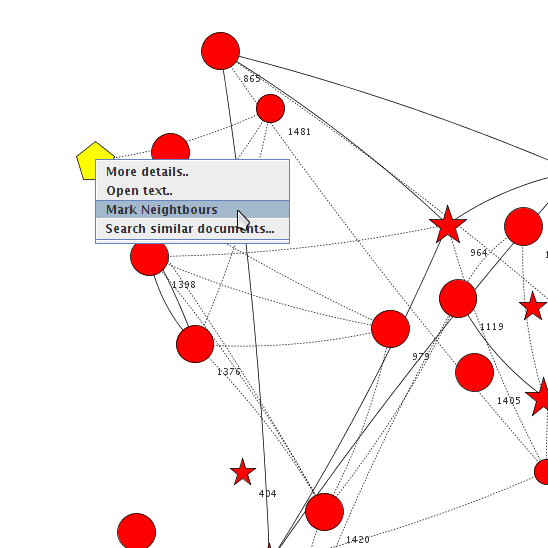
\includegraphics[width=80mm]{markneighbors_before.png}}
\subfloat[][After]{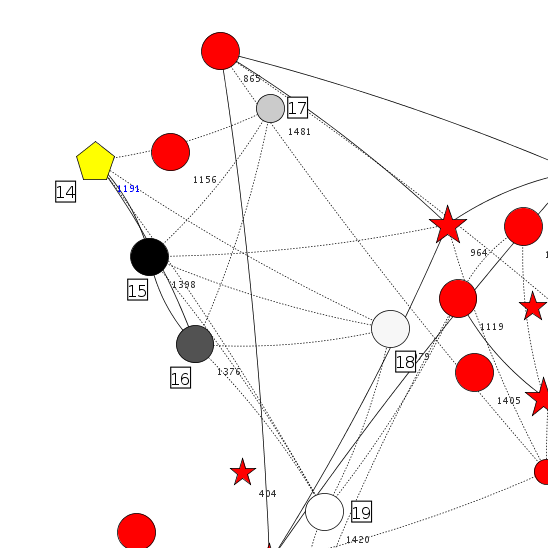
\includegraphics[width=80mm]{markneighbors_after.png}}
\end{figure}

Each nearest neighbor is automatically shaded in a range from black to white to represent the level of similarity between the node and the originally-selected node (item 14): The darker the shade, the more similar the document is to the document of the originally-selected node in relation to the other nearest neighbors; The lighter the shade, the less similar the document is. For example, of the nearest neighbours, item 15 is most similar to the originally-selected node. In descending order of similarity, the next most similar documents are item 16, 17 18 and 19.

\paragraph{Display Options}
\subparagraph{Edge/Node Filtering}

\begin{figure}[ht]
\centering
\caption{Display Options}
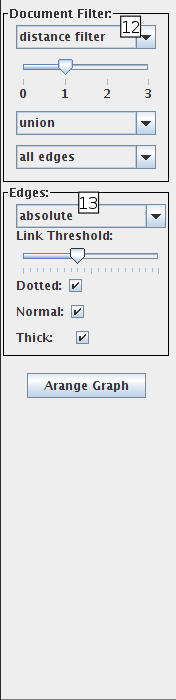
\includegraphics[height=80mm]{displayopts.png}
\end{figure}

The graphical display may be further adjusted by applying a distance filter (item 12) or by adjusting the method by which edges are drawn (item 13).

By default, the edges drawn are determined by the absolute similarity measure: If the similarity measure of two documents is greater than a user-adjustable edge threshold, an edge is drawn between them. The higher the absolute similarity of the two documents, the thicker the edge. However, the user may set the method of edge generation to display edges according to the relative similarity of the documents shown: According to the user-specifiable edge density, the more similar two documents are compared to the similarities of other documents, the thicker the edge.

By adjusting the edge threshold (for absolute similarity) or the edge density (for relative similarity) the user can adjust the level of detail represented by the graph. This allows the user to both discern relationships between documents which are not very similar to each other, and to prune out relatively weaker relationships between documents which are very similar to each other.

Likewise, a vertex filter may be applied, enabling the user to display only nodes of a specified distance $\leq x$ from a selected node or nodes, e.g.\ displaying only the nodes directly connected to the current node(s) (a distance of 1) or displaying nodes which are connected to the selected node through at most one other node (a distance of 2). When selecting multiple nodes, the user can select to display either the union of the neighbors, e.g.\ to display the nodes with a distance of $\leq x$ from \emph{any} selected node, or the intersection of the neighbors, e.g.\ to display only the nodes with a distance of $\leq x$ to \emph{all} selected nodes.

This may be done in real-time, i.e.\ after applying a distance filter, the user may select a node in the graph to view an updated graph of all nodes satisfying the distance criterion for the newly-selected node. This feature allows the user to explore ``sub-graphs'' of the main graph in real-time, allowing the user to focus on a particular cluster of documents and thus allowing the user even greater control over the search results.

\subparagraph{Advanced Options}
Finally, for even further control, the user may manually specify all display settings through the \scare{Setup} menu.

\begin{figure}[ht]
\centering
\caption{Advanced Settings}
\subfloat[][]{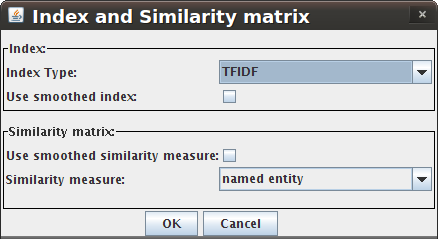
\includegraphics[scale=0.33]{menu_matrices.png}}\quad
\subfloat[][]{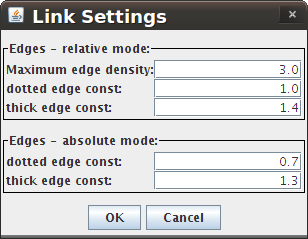
\includegraphics[scale=0.33]{menu_links.png}}\quad
\subfloat[][]{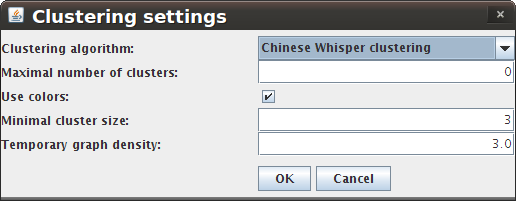
\includegraphics[scale=0.33]{menu_clustering.png}}
\end{figure}

\begin{description}
\item[\scare{Index and Similarity Matrix}] \hfill \\
The user can choose to have document similarities calculated with TF/IDF measures (default) or simply TF scores. Additionally, similarities may be calculated with aliasing through the string kernel, or to calculate document similarities with aliasing disabled and associating only exact strings (default). Finally, the similarities can be calculated using only NEs (default), only lexical similarity, or may manually specify the weighting of each measure individually (\scare{custom}), e.g.\ of each type of NE compared to each other and to overall lexical similarity. 
\item[\scare{Link Settings}]\hfill \\
The edge density slider on the left-hand control panel left corresponds to the edge density value in relative-similarity mode, or the edge threshold value in absolute-similarity mode. When the graph is constructed in the relative similarity mode, the number of edges is determined by multiplying the number of nodes by the the chosen edge density (slider value), and the strongest edges are displayed according to this value. After the set of edges is determined, the mean of the edge strength is computed. The strength of each edge is then compared with the mean of the edge strength. The ratio between the edge strength and the mean of the edge strength determines whether the edge will be dotted, normal or thick.

\begin{itemize}
\item \scare{Maximum edge density}: determines which density value corresponds to the right corner position of the density slider.

\item \scare{Dotted edge const}: If the edge strength is lower than the mean of the edge strength multiplied by dotted edge constant, then the edge is dotted.

\item \scare{Thick edge const} If the edge strength is higher then the mean of the edge strength multiplied by thick edge constant, then the edge is thick.
\end{itemize}

The following settings control the edge appearance in absolute-similarity mode:

\begin{itemize}
\item \scare{Dotted edge const}: If the strength of the edge lies between the dotted edge threshold and the normal edge threshold, then the edge is dotted.
\item \scare{Thick edge const}: If the strength of the edge is greater than the thick edge threshold, then the edge is thick.
\end{itemize}

If the strength of the edge lies between the normal edge threshold and the thick edge threshold, then the edge is normal.

The threshold value for normal edges is determined by the slider in the main control panel. The dotted-edge threshold value is then computed as a product of the normal edge threshold and the dotted edge constant. Likewise, the thick-edge threshold value is computed as a product of the normal edge threshold and the thick edge constant.
\item[\scare{Clustering Settings}] \hfill \\
The user can enable Chinese Whispering (CW) automatic document clustering (disabled by default), and specify the maximum number of clusters formed, the minimum size of each cluster, as well as the temporary graph density. Temporary graph is the data structure that is used for computation of the clusters. For the purpose of the clustering algorithm it's better to have dense graph, while users prefer rather sparser graph. That's the reason why there is a temporary graph structure for the purpose of the clustering algorithm. 
Clustering can be enabled by setting the maximum number of clusters to the positive value.
We implemented a modified version of Chinese Whispering algorithm. Modified algorithm is less overgenerating. It puts the document to the cluster only when there is a strong evidence. By increasing the "Activation threshold multiplier" and by decreasing the "Init iterations" algorithm becomes more conservative and vice versa. 
\end{description}

All of these features combine to create a powerful interface for searching the corpus and visualizing the results which is both highly automated and highly customizable. In turn, the system is designed to accommodate both basic and advanced users.

=======
\subsection{Data}\label{sec:data}
\subsubsection{Corpus Description}\label{sec:description_of_the_castro_archive}
\paragraph{Structure}
The \citeA{CastroDB} (CSDB) is an online corpus consisting of speeches, interviews, press conferences and other oratory by Fidel Castro from 1959 to 1996 translated into English, maintained by the Latin American Network Information Center (LANIC) at the University of Texas at Austin. The collection contains 1492 documents with an average document size of approximately 3,800 words. The information is presented as plain-text documents embedded into HTML web pages organized by the year and month of the original release. The documents are annotated with metadata including:

\begin{itemize}
\item The type of document (e.g.\ \scare{speech}, \scare{interview}, \scare{press conference})
\item The exact date of the original release
\item The author, e.g.\ Castro himself or a particular reporter
\item The original source, e.g.\ \scare{Havana Domestic Radio}
\item A headline (such as in a newspaper)
\item The reporting agency, e.g.\ the Foreign Broadcast Information Service (FBIS)
\item The exact date of the report
\end{itemize}

\paragraph{Linguistic properties}
The documents are manually translated from modern Spanish into modern English, sparing us many problems associated with documents written in historical languages. This characteristic, along with a considerable amount of newspaper comparable content allow a relatively straightforward application of technologies already deployed and currently used in NLP and IR.

However, the corpus is very heterogeneous: Not only does it span 37 years of oratory, but it also incorporates many different authors. Although it is a database dedicated to the oratory of Fidel Castro, it features many documents which are not narrated by Castro, for instance by news reporters, journalists and interviewers. Likewise, the corpus comprises many different genres and styles.

Secondly, many of the documents in the corpus are (at least indirectly) based on spoken language and so are not structured in a formal way, in polar opposition to e.g.\ a scientific report. Likewise, many documents in the corpus feature heavily-rhetorical content. Due to this characteristic, in many documents, topics are multiple and often vague. This observation is valid for the whole documents as well as smaller sections such as single paragraphs. 

In this way, the corpus is less similar to relatively-structured corpora (such as the Wall Street Journal-based \citeauthor{PTB}) it is to less-structured and more heterogeneous literary corpora. On these kinds of documents, topic identification as well as document summarization and clustering is difficult to implement manually (using human competence), let alone doing so automatically.

\subsubsection{Reading and Storing the Data}\label{sec:reading_and_storing_the_data}
\note{reading the data, creating MySQL database, creating data model}

At a first step we used a \texttt{shell}\footnote{http://tiswww.case.edu/php/chet/bash/bashtop.html}
script and \texttt{wget}\footnote{http://www.gnu.org/software/wget/} to download the complete castro
speech database. The actual speech data consists of a set of static webpages sorted by year into
folders. In a second processing step we parsed these html-files and extracted the actual content of
each file and its meta-information into textual format. To this end, several \texttt{shell} and
\texttt{python}\footnote{http://www.python.org/} scripts have been written.

The extracted information serves as the basis for the consecutive analysis and processing steps. In
order to provide structured access to the meta-information we developed a
\texttt{perl}\footnote{http://www.perl.org/} script to convert the meta-information for each
document into an entry in a \texttt{mysql}\footnote{http://www.mysql.de/products/enterprise/}
database. For every document, the database provides the following information
\begin{itemize}
 \item{\textsc{Author:} Name of the author of the document.}
 \item{\textsc{Location:} The place the document orginated.}
 \item{\textsc{Headline:} The headline of the document.}
 \item{\textsc{Date:} The date the document orginated.}
 \item{\textsc{ReportDate:} The date th3e content of the document appeared in written from.}
 \item{\textsc{Type:} There are several different types of documents in the databse. E.g.
 \texttt{SPEECH}, \texttt{INTERVIEW}, \texttt{ARTICLE}, etc.}
 \item{\textsc{Header:} Additional meta-information}
 \item{\textsc{Source:} The source where this document appeared in written form the first time.}
\end{itemize}
In addition to this information, we later enriched the database with the extracted named entities
(see \ref{sec:named_entity_recognition}) for each document. The columns \textsc{Persons},
\textsc{Places}, \textsc{Organizations} have been added and each field contains the bulk information
of the identified named entities as a comma separated list. Although this representation is is not
the most elegant and optimal solution, the derived database provides sufficient performance and
usability for the task at hand.

\subsection {Named Entity Recognition}
\label{sec:named_entity_recognition}
Please recall, that our ultimate goal is to come up with a cross-document recommendation system for
the castro speech database. Therefore, we need an appropriate metric on between document
similarity that serves as a basis for the recommendation software.

Our first idea was to use proper \textit{co-reference resolution}, e.g. provided by
\texttt{BART}\footnote{http://www.bart-coref.org/} software \cite{bart}. In this case, document
similarity is a function of the number of co-references that appear between two docuemnts. However,
in the end we decided to drop this approach because of the overall complexity and the tight time
constraints. In general, between document co-reference resolution far from an easy task. The castro
database though has some nice properties that allow for a more straightforward solution. For this
dataset, the domain is rather limited and the number of distinct topics should be small. Hence, we
came up with the idea to base the similarity measure on smoothed co-occurences of named entities.

The next step in the pre-processing chain is thus the execution of named entity recognition followed
by a smooting of the features in the vector space induced by the named entities using kernel
methods (see \ref{sec:string_kernel}) \cite{string_kernel_coref}.
\subsubsection{The Stanford Named Entity Recognizer}\label{sec:stanford_named_entity_recognizer}
\note{identifying names, locations and organizations in the Castro documents,
input/output examples, evaluation??}

YEVGENI WILL WRITE

CARSTEN - PROVIDE STATISTICS TABLE, WRITE ON TECHNICALITIES WITH RUNNING THE NER AND STORING RESULTS
\begin{figure}[ht]
\centering
\caption{Global statistics for the named entities. The table shows the number of distinct named
entities found by the stanford named entity recognizer and the average number of occurences for
each NE type per document.}
\begin{tabular}{l|ll}
  Named Entity Type      & Number & Average/Document\\
  \hline
  \textsc{Person}        & 6515   & 21.5\\
  \textsc{Organizations} & 3667   & 44.7\\
  \textsc{Locations}     & 6612   & 17.1\\
\end{tabular}
\label{fig:ne_statistics}
\end{figure}

For the subtask of named entity extraction we used the Stanford named entity recognizer (sNER)
\cite{sner} version $1.1.1$. The package provides several pre-trained classifiers trained on both US
and UK newswire data from CoNLL, MUC6, MUC7 and ACE.

The named entity recognition was performed with the
\texttt{ner-eng-ie.crf-3-all2008-distsim.ser.gz} model - a three class classifier for the named
entities \textsc{Person}, \textsc{Organizations} and \textsc{Locations} with an additional
``distributional similarity lexicon'' for improved performance. Processing was done by a
\texttt{shell} script that runs sNER for each document in the castro database. The input is a
textfile containing the content of a document without meta-information. For the output format we
choose a XML dialect.



\subsection{Representing Documents in Vector Space}\label{sec:representing_documents_in_vector_space}
MICHAL 

\subsubsection{Indexing}
\label{sec:indexing_term_weighting}
\note{description and motication of the 4 different representations}

\subsubsection{Term Weighting}
\label{sec:term_weighting}
\note{ tf/tfidf with motivation and
interpretation for each, examples}

Vector model is the model of representing text document or any other data. In vector model for information retrieval both documents and queries are represented as a vector of numbers. Number at each position of the vector corresponds to the term importance for the representation of the query or document. The main advantage of the vector model is that it has easy algebraic formulation. It's also not that strict as the boolean model. In boolean model document either completely fits to the query or it doesn't fit at all. In real word the situation is different, the relevance of the document for the user is rathed continuous quantity and the same applies to the vector model.

The coefficients are usually normalised in order to have the same length, otherwise the model would favor the documents with greater length. What is important is the density of the term in the document.

There are several measures beeing used which express the importance of the index term for the document. The most widely used are TF and TF-IDF. 
TF stands for term frequency, it measures directly how many times the word occured in the document, TF score grows linearly with the number of occurences of the term in the document. The TF score of term j in document i is defined as follows:

\note{Someone who can work with latex please add the following: $text{TF}(i,j) = n(i,j)$ / SUM(k
over all terms) n(i,k) }
\[\text{TF}(i,j) = n(i,j) / \sum_{k \in \mathcal{T}}{n(i,k)}\]

$n(i,j)$ stands for the number of counts term $j$ occured in document $i$.

TF-IDF stands for term frequency - inverse document frequency. This measure is based on the notion that the terms which occur in a lot of documents are not very useful for searching purposes. The terms which occur in a few documents only have greater discrimination power. The TF-IDF score of term j in document is is defined as follows.

\note{Someone who can work with latex please add the following: TF-IDF(i,j) = TF(i,j) * log( |D| /
\{d: t(j) "is member of sign" d\} }
\[\text{TF-IDF}(i,j) = \text{TF}(i,j)\log{(|D| |\lbrace d : t(j) \in d \rbrace|)}\]

The TF-IDF score of term j drops according to the logarithm of the number of document that contain term j. The TF-IDF score of the term which is contained in every single document is always equal to zero.

\note{The indexes in brackets should be written in foot-script, I hope you show me tomorrow how to write formulas:) }  

In vector model we need to measure the similarity between vectors. The similarity is usually expressed by the cosine similarity measure:

\note{ cosim(q,d) = [SUM(k over all terms) q(k) * d(k)] / [ |q| * |d| ] }
\[\text{cosim}(q,d) = \sum_{k \in \mathcal{T}}\frac{q(k)d(k)}{|q||d|}\]

It express the cosin angle between the vectors q and d. This measure is equal to 1 for the paralell vectors and it's equal to zero for the perpendicular vectors.

In vector model the searching proceeds as follows. The search query is transformed into its vector representation in the same manner as it is done for the document. The cosine similarity between the query vector and the vector representation of each document is computed. The search results are ordered according to their similarity to the user query.  

Vector representations of the documents are stored in the index matrix. Each row of the index matrix corresponds to the vector representation of a single document. 

Our model contains several index matrix. We created index matrix for each named entity type and also index matrix for general index which indexes the non named entity terms. For all named entity types aliased or non-aliased index matrix can be used. Our current implementation of vector model doesn't use TF-IDF measure for adjustment of query terms. It means that all the values corresponding to the search terms in the query are the same in the vector representation of the query. In the future we would like to implement proper TF-IDF weighting of the query terms. \note{Check whether the TF-IDF weighting of query terms is common praxis} We would also like to implement query expansion using the string kernel. In current implementation query term must match exatly the named entity in the database otherwise the search term is not taken into the account. String kernel expansion would allow us to match query named entity with the named entity stored in the index file even when they don't match perfectly. In the current version query terms which are named entities must also have the proper capitalization.

Document retrieval in our model consists of two steps. In the first step, document, that don't satisfy the condition concerning the type and date of the document, are filtered out. In the second step documents are sorted in descending order according to their cosine measure similarity with the query. Only the subset of the best results of the size specified by the user proceeds to the next stage.


\subsubsection {Aliasing with String Kernels}
\label{sec:aliasing_string_kernel}
\note{motivation, description of the algorithm to create similarity matrixes between NE's,
smoothing document representations with Kernel matrix as aliasing}



\subsection{Information Retrieval}\label{sec:information_retrieval}
\subsubsection{Keyword Search}\label{sec:keyword_search}
\note{description of the functionality, use of string kernels for query expansion }

\subsubsection{Metadata Search}\label{sec:metadata_search}
\note{general description of the functionality}

\subsection{Computing Similarity between Documents}\label{sec:computing_similarity_between_documents}
\input{documentsimilarity}

\subsection{Graphical Representation}\label{sec:graphical_representation}
\subsubsection{Computing Graph Layouts}
So far we have described how nodes and edges of the graph are obtained from documents and their
similarity. In order to display the graph, a graph layout (two dimensional representation of the
graph) must be determined. If the vector representation of the document is only two dimensional,
then it is straightforward to obtain the graph layout just by using the features as two dimensional
coordinates. However, the documents in our model are represented by vectors with several thousands
of dimensions. The problem of reducing the dimensionality, is usually not solved by mapping
from high dimensional vector space to the low dimensional vector space but by using algorithms that
solve the problem of graph layouting directly using only the properties of the underlying graph
(nodes and edges together with their weights).

The layouting algorithm that was used in this project belongs to the popular class of force-based
layout algorithms which are based on physical modeling. An Edge is considered a spring and
the nodes are considered to be electrically charged particles (i.e.\ with equal signed charge such
that they repel each other) The optimal length of the springs is set in advance. Springs whose
length is larger or smaller than their optimal length exert a force that acts on the connected
nodes. In each iteration of the layouting algorithm, nodes are moved according to the resultant
force
that acts on them. After some time the position of the nodes becomes (quasi) stationary and the
system get into a local equilibrium state.

The described class of force based layout algorithms subsumes various algorithms with different
properties. However, they all perform variations of force-field energy minimization by iterative
approximation schemes. In this project the very basic algorithm as it is described in the previous
paragraph was used.

\subsubsection{Jung Graph Framework}
For the purpose of graph layouting, graph painting and user-graph interaction, the
\texttt{Jung\footnotemark{http://jung.sourceforge.net/} - java universal network/graph framework}
was used. It provides great flexibility in adjusting the graph appearance. Several so-called
transformers which affect node and edge label appearance can be plugged together to result in the
aesthetically pleasant appearance. \texttt{Jung} also provides predefined classes that allow for
easy interaction with the user. Functionalities for graph translation, zooming, node selection, node
transposition and other features can be achieved with minimal programming effort. One notably
strong point of the library is its template based design with the possibility to include several
plug-in components such as rendering and transformers that affect the resulting appearance of the
graph.

However there are some aspects of the \texttt{Jung} library, that were annoying fro the project.
First, it is difficult to achieve certain low level functionalities, like e.g.\ monitoring the
on-screen position of a fixed point while translation of the graph was performed. Secondly, several
operation are implemented in a circumstantial way. For example, in order to change the color of
one node the whole graph must be redrawn and during this process all active visualization
transformers are applied on each graph object.When we used the default implementation of the
\texttt{Jung} visualization class, the application consumed more then 50\% of the processor time
even though there was no ongoing user interaction or computation task (this depended on the size of
the presented graph --- the statement holds for graph with 25 nodes about 50 edges). By extending
the standard \texttt{Jung VisualizationViewer} class and overriding several functions, the issue of
unnecessary graph redrawing was resolved and accordingly the problem of the low gui performance.

\subsubsection {Querying Functionalities}
\label{sec:querying_functionalities}
The nodes of the graph are generated from the results of a database query supplied by the user, who
can search either by keyword, by NE, or by a combination of both in the same query. Likewise, the
user may select a range of years to search in (e.g.\ retrieve documents occurring between
\code{1970} and \code{1975}), as well as select only certain types of documents to be searched
(e.g.\ retrieve only documents of type \meta{Speech} or \meta{Interview}). The documents most
relevant to the current query are displayed, the number of the documents displayed being specified
by the user (e.g.\ display the \code{25} most relevant documents), and edges connecting each
document are drawn based on the similarity measures relating each document to each other.

\subsubsection {Presenting Results}
\label{sec:presenting_results}
After submitting a query, a table of query results is displayed and a graph corresponding to the
results is drawn, in which the relevance measure of each document to the current query is
represented by the absolute size of the node representing the document in question: The larger the
node, the more relevant it is to the current query. The type of document represented by the node is
represented by its shape, e.g.\ \meta{Speech} $\rightarrow$ star, \meta{Meeting} $\rightarrow$
pentagon. The edges linking the nodes of the graph represent the strength of similarity the of the
two documents represented by the nodes.
	
\subsection{Combining It All: User Interface}\label{sec:combining_it_all:_user_interface}
The query functions, graph and display functions are integrated into a single graphical front-end relying primarily on the mouse for user input. The graph representation is dynamic and interactive, able to be navigated through by the user in order to obtain detailed information regarding the document database.

\begin{figure}[ht]
\centering
\caption{GUI}
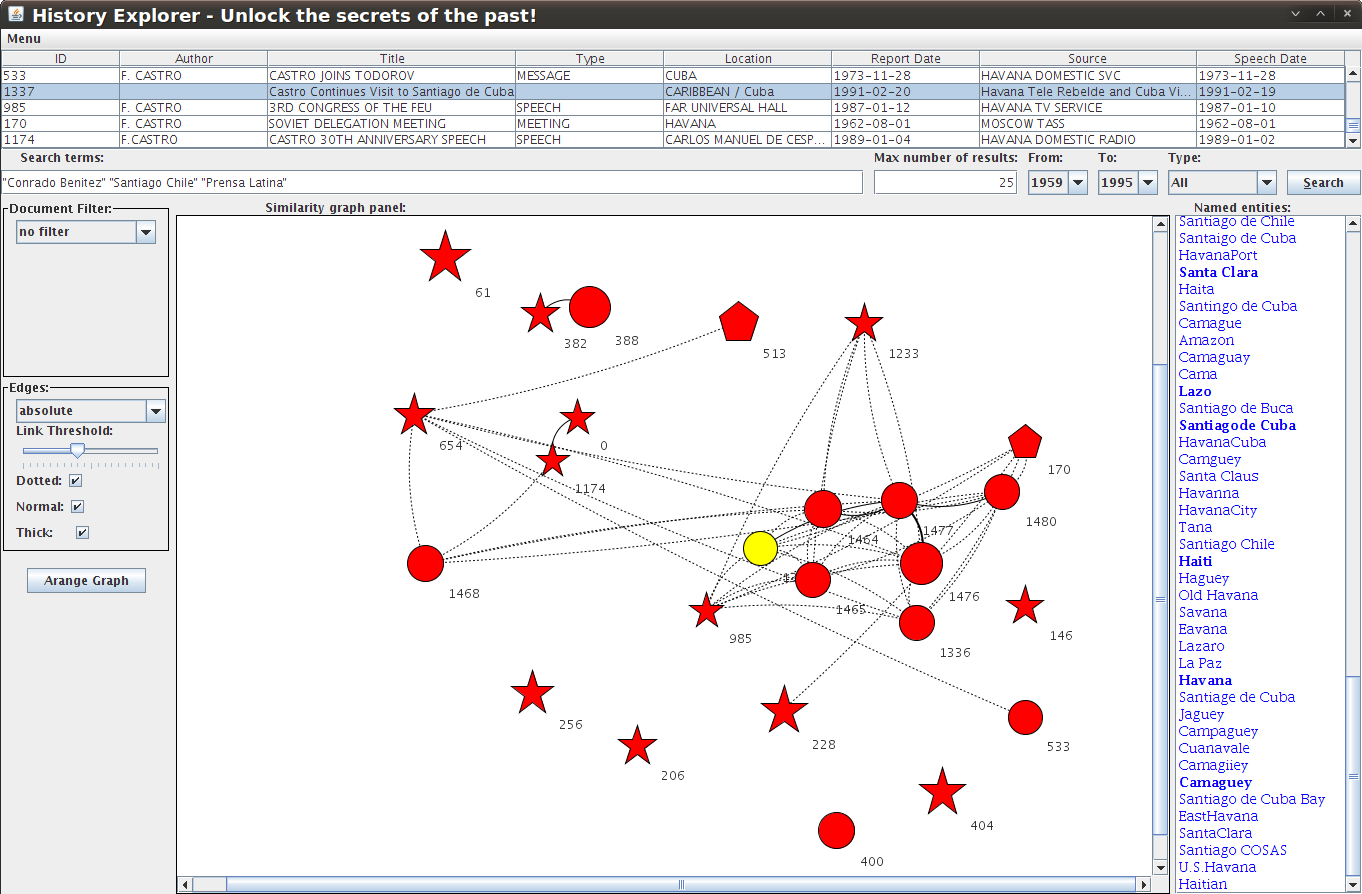
\includegraphics[width=160mm]{gui.png}
\end{figure}

\subsubsection{Search Function}
\begin{figure}[ht]
\centering
\caption{Search query}
\subfloat[][~\hfill{\tiny Version $<$\code{2010-04-02}}]{

\includegraphics[width=160mm]{search.png}
}
\end{figure}

Search terms are entered in the query form (item 1 in the figure above)\footnote{Unless otherwise mentioned, the version depicted is \code{2010-04-02}.}: Entering any term will return both NEs and also keywords sharing the exact form (not case-sensitive)--- For instance, entering \lingform{committee} will both return exact instances of \code{committee} in the document itself, and will return NEs similar to \lingform{committee} based on the string kernel similarity measure, e.g.\ \lingform{Central Committee} and \lingform{Central Committee of the Cuban Communist Party}. Multi-word terms are denoted in double quotes, e.g.\ \code{"Central Committee"}. The maximum amount of query results can be adjusted (item 2): For example, entering a value of \code{10} will return ten documents most relevant to the query. The set of years searched between is also modifiable specified by (item 3), as well as the type(s) of documents searched (e.g.\ \code{Speech}, \code{Interview}) (item 5). Once the criteria are entered, the query is run by selecting item 5.

\paragraph{Presentation}
The results of the current query are displayed both in a table of results and in a graph displayed in the main window.

\subsubsection{Visualization of Results}
\begin{figure}[ht]
\centering
\caption{Query Results Table}
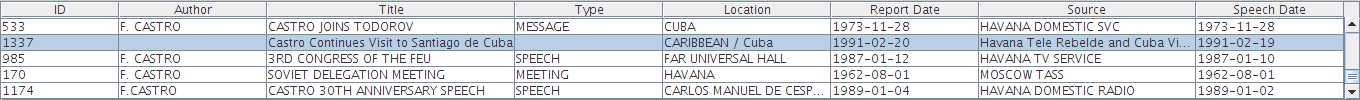
\includegraphics[width=160mm]{table.png}
\end{figure}

In the table, the documents are displayed in rows sorted by their relevance to the query in descending order. The metadata associated with each document is displayed in columns. If there was no metadata retrieved for a document, the entry for the data is empty or \code{NULL}.

\begin{figure}[ht]
\centering
\caption{Document Similarity Graph}
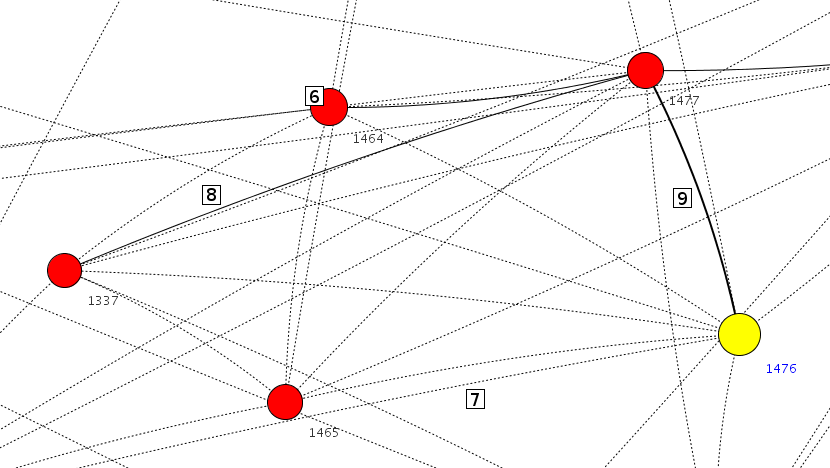
\includegraphics[width=80mm]{nodecloseup.png}
\end{figure}

In the graph, each document is represented by a node (item 6). The relevance of the document to the query is represented by the size of the node: The larger the node, the more relevant the document is to the submitted query. The edges between the nodes represent similarities between the documents based on the similarity of the two documents based on the NEs each contain and their aliases according to the string kernel measure. The stronger the similarity connection, the heavier the line weight of the edge drawn. There are three line weights: ``dotted'' (item 7), ``normal'' (item 8) and ``heavy'' (item 9), in ascending order of the level of similarity they represent. The graph can be scaled in real-time by zooming in and out with the scroll wheel. Furthermore, it is able to re-arrange the position of each node in the graph by clicking and dragging them in order to optimize the view of the graph manually. The graph can also be set to re-arrange the nodes automatically by clicking ``Arrange Graph''. By pressing CTRL and clicking on a node, the view will be centered on the said node automatically.

\paragraph{Navigation}
Selecting a document either through its corresponding entry in the table or node in the graph with the mouse or keyboard highlights it and displays the NEs in the document in a sidebar. The NEs in a particular document and their string kernel-based aliases are displayed in the sidebar: Boldface entries represent NEs in the given document, while the non-boldface entries represent NEs similar to the boldface NEs in the document according to the string kernel similarity measure. For example, the NE \textbf{\lingform{Castro}} may also return the similar NEs \lingform{Fidel}, \lingform{Fidel Castro} and \lingform{Dr.\ Fidel}. The type of the NE (e.g.\ \meta{person} or \meta{organization}) is represented by the color of the text, e.g.\ red for \meta{Persons}, green for \meta{Organizations} and blue for \meta{Locations}. It also is possible to select multiple documents, e.g.\ by holding SHIFT and clicking on multiple nodes/table entries, or by clicking and dragging the mouse to create a selection box encompassing the nodes/table entries to be selected. When multiple documents are selected, the entries displayed in the sidebar are those that are common to all selected documents.

\begin{figure}[ht]
\centering
\caption{Node Context Menu}
\subfloat[][~\hfill{\tiny Version $<$\code{2010-04-02}}]{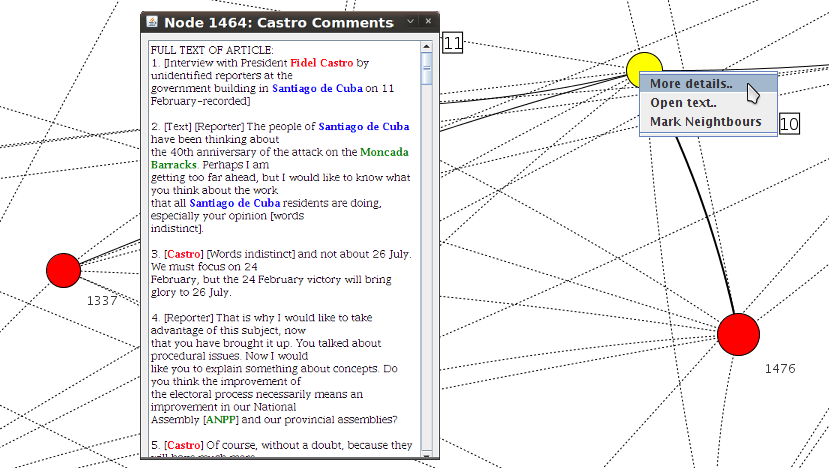
\includegraphics[width=80mm]{nodeclick.png}}
\end{figure}

In addition to viewing document metadata in the query results table, the user may to view the metadata of the document associated with a particular node (e.g.\ document \meta{Type}, \meta{Date} or \meta{Location}) through the node's context menu (item 10) (i.e.\ by right-clicking on the node with the mouse). Also available through the context menu is the text of the document itself, which is displayed in a separate window which can be kept open while still navigating through the graph and viewing other nodes (item 11). The NEs in the text are denoted by being colored according to their type.

\paragraph{\scare{Mark Nearest Neighbors} Function}
Lastly, it is possible through the context menu to automatically select the nearest neighbors of the selected node(s), i.e.\ to select the nodes which share a NE directly with the said node.

\begin{figure}[ht]
\centering
\caption{\scare{Mark Nearest Neighbors} Function}
\subfloat[][Before]{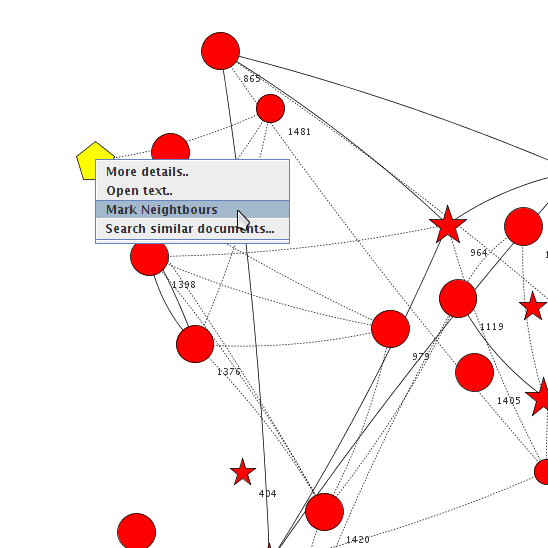
\includegraphics[width=80mm]{markneighbors_before.png}}
\subfloat[][After]{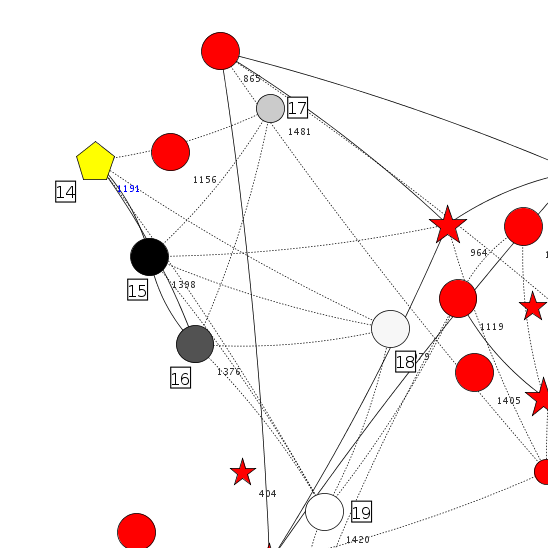
\includegraphics[width=80mm]{markneighbors_after.png}}
\end{figure}

Each nearest neighbor is automatically shaded in a range from black to white to represent the level of similarity between the node and the originally-selected node (item 14): The darker the shade, the more similar the document is to the document of the originally-selected node in relation to the other nearest neighbors; The lighter the shade, the less similar the document is. For example, of the nearest neighbours, item 15 is most similar to the originally-selected node. In descending order of similarity, the next most similar documents are item 16, 17 18 and 19.

\paragraph{Display Options}
\subparagraph{Edge/Node Filtering}

\begin{figure}[ht]
\centering
\caption{Display Options}
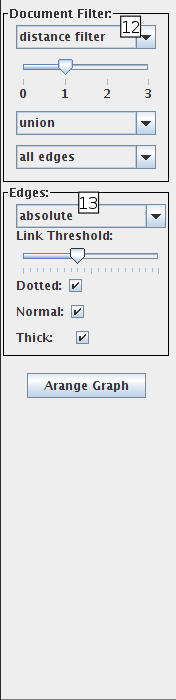
\includegraphics[height=80mm]{displayopts.png}
\end{figure}

The graphical display may be further adjusted by applying a distance filter (item 12) or by adjusting the method by which edges are drawn (item 13).

By default, the edges drawn are determined by the absolute similarity measure: If the similarity measure of two documents is greater than a user-adjustable edge threshold, an edge is drawn between them. The higher the absolute similarity of the two documents, the thicker the edge. However, the user may set the method of edge generation to display edges according to the relative similarity of the documents shown: According to the user-specifiable edge density, the more similar two documents are compared to the similarities of other documents, the thicker the edge.

By adjusting the edge threshold (for absolute similarity) or the edge density (for relative similarity) the user can adjust the level of detail represented by the graph. This allows the user to both discern relationships between documents which are not very similar to each other, and to prune out relatively weaker relationships between documents which are very similar to each other.

Likewise, a vertex filter may be applied, enabling the user to display only nodes of a specified distance $\leq x$ from a selected node or nodes, e.g.\ displaying only the nodes directly connected to the current node(s) (a distance of 1) or displaying nodes which are connected to the selected node through at most one other node (a distance of 2). When selecting multiple nodes, the user can select to display either the union of the neighbors, e.g.\ to display the nodes with a distance of $\leq x$ from \emph{any} selected node, or the intersection of the neighbors, e.g.\ to display only the nodes with a distance of $\leq x$ to \emph{all} selected nodes.

This may be done in real-time, i.e.\ after applying a distance filter, the user may select a node in the graph to view an updated graph of all nodes satisfying the distance criterion for the newly-selected node. This feature allows the user to explore ``sub-graphs'' of the main graph in real-time, allowing the user to focus on a particular cluster of documents and thus allowing the user even greater control over the search results.

\subparagraph{Advanced Options}
Finally, for even further control, the user may manually specify all display settings through the \scare{Setup} menu.

\begin{figure}[ht]
\centering
\caption{Advanced Settings}
\subfloat[][]{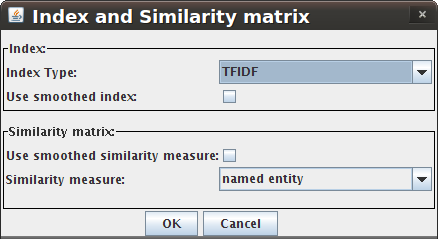
\includegraphics[scale=0.33]{menu_matrices.png}}\quad
\subfloat[][]{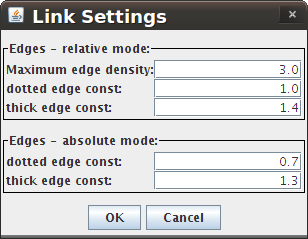
\includegraphics[scale=0.33]{menu_links.png}}\quad
\subfloat[][]{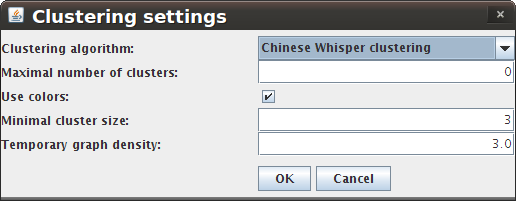
\includegraphics[scale=0.33]{menu_clustering.png}}
\end{figure}

\begin{description}
\item[\scare{Index and Similarity Matrix}] \hfill \\
The user can choose to have document similarities calculated with TF/IDF measures (default) or simply TF scores. Additionally, similarities may be calculated with aliasing through the string kernel, or to calculate document similarities with aliasing disabled and associating only exact strings (default). Finally, the similarities can be calculated using only NEs (default), only lexical similarity, or may manually specify the weighting of each measure individually (\scare{custom}), e.g.\ of each type of NE compared to each other and to overall lexical similarity. 
\item[\scare{Link Settings}]\hfill \\
The edge density slider on the left-hand control panel left corresponds to the edge density value in relative-similarity mode, or the edge threshold value in absolute-similarity mode. When the graph is constructed in the relative similarity mode, the number of edges is determined by multiplying the number of nodes by the the chosen edge density (slider value), and the strongest edges are displayed according to this value. After the set of edges is determined, the mean of the edge strength is computed. The strength of each edge is then compared with the mean of the edge strength. The ratio between the edge strength and the mean of the edge strength determines whether the edge will be dotted, normal or thick.

\begin{itemize}
\item \scare{Maximum edge density}: determines which density value corresponds to the right corner position of the density slider.

\item \scare{Dotted edge const}: If the edge strength is lower than the mean of the edge strength multiplied by dotted edge constant, then the edge is dotted.

\item \scare{Thick edge const} If the edge strength is higher then the mean of the edge strength multiplied by thick edge constant, then the edge is thick.
\end{itemize}

The following settings control the edge appearance in absolute-similarity mode:

\begin{itemize}
\item \scare{Dotted edge const}: If the strength of the edge lies between the dotted edge threshold and the normal edge threshold, then the edge is dotted.
\item \scare{Thick edge const}: If the strength of the edge is greater than the thick edge threshold, then the edge is thick.
\end{itemize}

If the strength of the edge lies between the normal edge threshold and the thick edge threshold, then the edge is normal.

The threshold value for normal edges is determined by the slider in the main control panel. The dotted-edge threshold value is then computed as a product of the normal edge threshold and the dotted edge constant. Likewise, the thick-edge threshold value is computed as a product of the normal edge threshold and the thick edge constant.
\item[\scare{Clustering Settings}] \hfill \\
The user can enable Chinese Whispering (CW) automatic document clustering (disabled by default), and specify the maximum number of clusters formed, the minimum size of each cluster, as well as the temporary graph density. Temporary graph is the data structure that is used for computation of the clusters. For the purpose of the clustering algorithm it's better to have dense graph, while users prefer rather sparser graph. That's the reason why there is a temporary graph structure for the purpose of the clustering algorithm. 
Clustering can be enabled by setting the maximum number of clusters to the positive value.
We implemented a modified version of Chinese Whispering algorithm. Modified algorithm is less overgenerating. It puts the document to the cluster only when there is a strong evidence. By increasing the "Activation threshold multiplier" and by decreasing the "Init iterations" algorithm becomes more conservative and vice versa. 
\end{description}

All of these features combine to create a powerful interface for searching the corpus and visualizing the results which is both highly automated and highly customizable. In turn, the system is designed to accommodate both basic and advanced users.

>>>>>>> aa4728359f3b98dec5ad7e63a89cff0d0cf69d13


\section{Evaluation}\label{sec:evaluation}
\note{FROM CAROLINE: Evaluation 
of sub-components and system overall (insofar as it makes sense) 
either quantitative (e.g., accuracy for information extraction 
task) and/or qualitative (e.g., give examples where your system 
improves IR over keyword-based search) 
also discuss cases where your system doesn't perform well and 
describe how it could be improved (error analysis)}

\subsection {Named Entity Recognition}
\label{sec:named_entity_recognition}

\subsection {String Kernels and Co-reference Resolution}
\label{sec:string_kernels_and_co-reference_resolution}

\subsection {Document Similarity}
\label{sec:document_similarity}

\subsection {Information Retrieval}
\label{sec:information_retrieval}

\subsection {GUI Performance}
\label{sec:gui_performance}
The results of the document similarity visualization are mixed: While there are many relationships represented between documents, the qualitative value of these relationships is irregular.

For example, a query including the named entity \code{"Central Committe"} and the keyword \code{economy} for documents between the years of 1959 and 1984 produced a cluster of documents including the following headlines:

\begin{enumerate}
\item ``USSR--Cuban Fishing Base Pact Signed''\label{eval:doc179}
\item ``Fidel Castro sends regrets to Dominican Olympic Committee''\label{eval:doc553}
\item A meeting of Fidel Castro with Salim Rabay'l `Ali, assistant secretary of the Central Committee of the United Political Organization National Front\label{eval:doc682}
\item A meeting of Fidel Castro with Jesse Jackson regarding US--Cuban normalization\label{eval:doc879}
\item A meeting of Fidel Castro with Mrs. Nguyen Thi Binh, minister of foreign affairs of the Republic of South Vietnam\label{eval:doc643}
\item An address by Fidel Castro to the people of Chile regarding Chilean--Cuban relations and working for a better future\label{eval:doc391}
\item Fidel Castro visits the South Vietnamese embassy in Cuba to welcome ``the great victory \ldots in liberating Saigon'' and inquire about social, economic and political conditions in South Vietnam\label{eval:doc626}
\end{enumerate} 

This cluster was obtained with a relative edge density of 2.52 (relatively high) while also applying a vertex distance filter of 1, selecting document \ref{eval:doc179} as a focal point. In other words, the graph was set to display many relations between all documents which shared at least one named entity with the document in question. Of the six documents connected to this document in the resulting graph (shown above), only one--- \ref{eval:doc626}--- is qualitatively related to document \ref{eval:doc179} in a direct sense.

However, all these documents contain the named entity \lingform{Central Committee} or a named entity similar to it according to the string kernel similarity measure. This is often realised as \lingform{First secretary of the \textbf{Central Committee} of the Communist Party of Cuba} or a variant of it--- which often co-refers to \lingform{Fidel Castro} or a variant of it.

It seems then that the document clustering is more relevant than first observed: All the documents contain references to \code{Fidel Castro}. However, this is still of little practical use, as the named entity \code{Fidel Castro} is in the vast majority of the documents in the corpus: This clustering does not distinguish a document or group of documents in a way which is of great use to a user browsing the corpus.

However, querying more specific terms revealed different results: Querying \code{"Giron"}, and \code{"Kennedy"} produced a graph of documents which are much more similar to each other in a qualitative sense than that produced by the previous query, for example:

\begin{enumerate}
\item ``Castro marks 5th anniversary of [Bay of Pigs] invasion'' \label{eval:doc274}
\item Speech for funeral of five Cuban troops killed in Baracoa landing operation [of the Bay of Pigs invasion]\label{eval:doc337}
\item ``Castro marks 2nd anniversary of [Bay of Pigs]'' invasion \label{eval:doc210}
\item An article on US--Cuban--Soviet relations, including consequences of ``Giron'' (the Bay of Pigs) and the Cuban Missile Crisis, mentioning President Kennedy\label{eval:doc864}
\item Report of the arrival of Algerian Preimier Ben Bella in Havana and Castro's speech for it--- in which he mentions the ``victory'' at ``Giron''
\item ``Castro discusses Latin America in EFE interview'', mentioning Kennedy and several of his actions regarding Latin America \label{eval:doc923}
\item ``Castro denounces U.S. aggression'' (April 1961) \label{eval:doc134} (regarding 
\end{enumerate} 

clustered most similar to document \ref{eval:doc134} anniversary speeches, edge density 2.52, distance 1.

7 total documents in cluster. All but one of them are directly related to the Bay of Pigs invasion itself, US aggression and/or President Kennedy. Even more interesting is that the document \ref{eval:doc337} was relatively isolated in the graph compared to the many edges connecting the anniversary speeches and politically-motivated documents such as \ref{eval:doc923,eval:doc134}.

\section{Conclusion}\label{sec:conclusion}
\subsection {Summary}
\label{sec:summary}

We presented a system that bla bla bla
TO BE COMPLETED


\subsection {Future Work}
\label{sec:future_work}
The presented system is a work in constant progress. 
In the following we present several ideas for possible improvements we plan to experiment with in future work.

TO BE EXPANDED
APLICABILITY OF APPROACH TO OTHER HISTORICAL DATABASES

\subsubsection{NLP processing}
For our current goals we limited ourselves to three kinds of named entities. 
It is however possible to extract additional relevant types of named entities. 
This direction can be further expanded with automatic extraction of events and other kinds of information that can be relevant for measuring 
document similarity in a historically motivated way.  

The proposed coreference resolution approach can be further expanded to include referring expressions. 
This is expected to have a positive impact on the reliability of the similarity measure. 
We also intend to experiment with an off-the-shelf coreference resolution system such as BART.
We plan to perform more thorough evaluation of each of the NLP dub tasks. 


\subsubsection{Visualization}
The visualization system can be further improved in several manners. 
A direction we intend to explore is the relevance and possibilities of plotting and representing correlations of the retrieved documents 
to different parameters, such as time and locations.

We also indent to experiment with additional graph layouts that have the potential of highlighting different properties of the 
retrieved set of documents. For example, we plan to implement a chronological layout, in which nodes are presented on a single chronological 
line. Edges will come in the form of arcs. Such representation has the potential of revealing time related information that is not 
directly visible in the current layout. 

As our representation comes in the form of a graph, a natural direction for futher exploration would be to examine the usefulness of 
graph algorithms for inferring interpretable information. One of the possibilities is to experiment with automatic clustering algorithm 
that would enable highligting clusters in the graph. 

Finally, we plan to perform several optimizations that would improve the real-time performance of our graphical user interface.  

We believe that enhancing the system in the proposed directions can further establish the relevance and usefulness of our tool for historians.  



\section{Appendix}

\bibliographystyle{apacite}
\bibliography{bib}
\end{document}